\documentclass[journal]{IEEEtran}
\usepackage{amsmath,amsfonts,amssymb}
\usepackage{array}
\usepackage{booktabs}
\usepackage[caption=false,font=normalsize,labelfont=sf,textfont=sf]{subfig}
\usepackage{textcomp}
\usepackage{stfloats}
\usepackage{url}
\usepackage{verbatim}
\usepackage{graphicx}
\usepackage{cite}
\usepackage{colortbl}
\usepackage{xcolor}
\usepackage{microtype}

\hyphenation{op-tical net-works semi-conduc-tor IEEE-Xplore}

\begin{document}

\title{QLoRA Distillation for Algorithmic Code Reasoning:\\ Addressing the ``Valley of Code Reasoning'' via Decoupled Algorithmic Conditioning}

\author{Pranav~Bhat~P~(231IT049),
        Shivam~Kumar~(231IT069),
        and~Himanshu~Mehar~(231IT027)%
}

% Paper headers
\markboth{IT488 Large Language Models Project Report,~Vol.~1, No.~1,~October~2026}%
{Bhat \MakeLowercase{\textit{et al.}}: QLoRA Distillation for Algorithmic Code Reasoning}

\maketitle

\begin{abstract}
Distilling competitive programming capabilities from frontier models into compact, sub-1B parameter student models is notoriously difficult. As documented by He et al. (2025), standard chain-of-thought code distillation exhibits a counter-intuitive scaling pathology known as the ``Valley of Code Reasoning'': at intermediate training volumes, student execution accuracy drops sharply before recovering at massive data scales. We attribute this performance trough to token entanglement---forcing a small language model to simultaneously choose high-level algorithmic strategies and emit low-level Python syntax within a single autoregressive pass. 

In this course project for IT488, we introduce a decoupled System-2 distillation architecture that splits problem solving into two explicit stages. First, a Stage~1 4-bit QLoRA classifier selects an algorithmic paradigm $P(\tau \mid \mathbf{X})$ across a 10-class taxonomy. Second, a Stage~2 code generator conditions its rationale and code synthesis on that predicted paradigm $P(\mathbf{C}, \mathbf{R} \mid \mathbf{X}, \tau)$. 

Up to our current 50\% milestone, we have built and verified: (1) a balanced 100-problem TACO benchmark across 10 algorithmic classes; (2) a sandboxed execution judge with POSIX resource limits (512\,MB RAM, 2.0\,s CPU); (3) a semantic rationale filter with a 91.0\% retention yield that discards misaligned teacher traces; (4) an unconditioned baseline ablation model; (5) an automated Pass@1 test suite; and (6) a class-balanced scaling partitioner ($10\%$, $25\%$, $50\%$, and $100\%$). Benchmarks on an NVIDIA Tesla T4 GPU demonstrate the viability of our 4-bit QLoRA setup: Stage~1 classification on Qwen2.5-0.5B reduces training loss from 5.38 to 0.77 within 44.6\,s, reaching 22.22\% Top-3 accuracy on 18 unseen test problems under extreme few-shot conditions (64 training samples), while Stage~2 fine-tuning on Qwen2.5-Coder-0.5B converges to a loss of 1.18 in 97.4\,s. These deliverables establish our end-to-end framework and pave the way for the full end-semester scaling sweep.
\end{abstract}

\begin{IEEEkeywords}
Large Language Models, Knowledge Distillation, QLoRA, Code Reasoning, Algorithmic Synthesis, Valley of Code Reasoning, Execution Sandboxing, Competitive Programming.
\end{IEEEkeywords}

\section{Introduction and Theoretical Motivation}
\IEEEPARstart{G}{enerating} correct algorithmic code is one of the most demanding tasks in applied machine learning. Unlike conversational dialogue or text translation, competitive programming problems from benchmarks like TACO \cite{li2023taco}, Codeforces, and AtCoder leave no margin for error. Candidate solutions must satisfy strict asymptotic complexity limits, exact input-output contracts, and obscure edge cases. A single off-by-one indexing mistake or an ill-suited container choice immediately results in an execution failure: Wrong Answer (WA), Time Limit Exceeded (TLE), or Runtime Error (RE).

\subsection{The Base Paper: Scaling Dynamics and the ``Valley of Code Reasoning''}
In a recent empirical investigation, He et al. (2025) \cite{he2025valley} uncovered an unexpected scaling pathology in code distillation, which they termed the \textbf{``Valley of Code Reasoning''}. When small student models are fine-tuned on reasoning traces from frontier teachers (such as DeepSeek-R1 or GPT-4o), functional correctness does not improve monotonically with training data volume:
\begin{enumerate}
    \item \textbf{Heuristic Baseline}: At low data regimes ($\approx 10\%$), students rely on simple syntax heuristics learned during pre-training, achieving modest baseline pass rates.
    \item \textbf{The Reasoning Valley}: At intermediate scales ($25\%$ to $50\%$), performance drops sharply. Students imitate verbose teacher rationales without grounding them in valid logic, leading to frequent syntax errors and execution timeouts.
    \item \textbf{Late Recovery}: Only at full data volume ($100\%$) does the student finally align rationale tokens with executable syntax.
\end{enumerate}

\subsection{Root Causes: Why Single-Stream Distillation Breaks Down}
We attribute this performance dip to three structural flaws in existing setups:
\begin{itemize}
    \item \textbf{Token Entanglement in Causal Attention}: Standard chain-of-thought distillation optimizes a single autoregressive objective, $\log P(\text{Rationale}, \text{Code} \mid \text{Problem})$. This forces a sub-1B model to interleave high-level algorithmic planning (System-2) with low-level Python syntax emission (System-1) inside the same causal attention stream.
    \item \textbf{Misaligned Teacher Supervision}: Frontier teachers often generate contradictory traces---describing a greedy approach in text while writing a dynamic programming matrix in code. Distilling conflicting tokens introduces high gradient variance into student adapters.
    \item \textbf{Resource Constraints in Academic Setups}: Most studies evaluate 7B to 32B models on multi-GPU clusters, leaving sub-1B models on single-GPU academic budgets largely unaddressed.
\end{itemize}

\subsection{Decoupled Algorithmic Conditioning Formulation}
We address this entanglement by decomposing code generation into two distinct stages:
\begin{equation}
\label{eq:decoupled}
P(\mathbf{C}, \mathbf{R} \mid \mathbf{X}) = \sum_{\tau \in \mathcal{T}} P(\tau \mid \mathbf{X}) \cdot P(\mathbf{C}, \mathbf{R} \mid \mathbf{X}, \tau)
\end{equation}
where $\mathbf{X}$ is the problem description, $\tau$ is an algorithmic paradigm from a 10-class taxonomy $\mathcal{T}$, $\mathbf{R}$ is the rationale, and $\mathbf{C}$ is the Python 3 code.

In practice, Stage~1 predicts the most likely paradigm $\tau^* = \arg\max_\tau P(\tau \mid \mathbf{X})$, and Stage~2 conditions generation on that explicit tag:
\begin{equation}
\label{eq:stage2_map}
\mathbf{C}^*, \mathbf{R}^* = \arg\max_{\mathbf{C}, \mathbf{R}} P(\mathbf{C}, \mathbf{R} \mid \mathbf{X}, \tau^*)
\end{equation}
This mirrors human competitive programmers, who identify the algorithm before writing code, freeing the generator to focus on correct syntax and edge cases. Fig.~\ref{fig:methodology} illustrates the complete architectural methodology, tracing the flow from raw benchmark tasks to teacher trace curation, two-stage student distillation, and isolated sandbox execution.

\begin{figure}[!b]
\centering
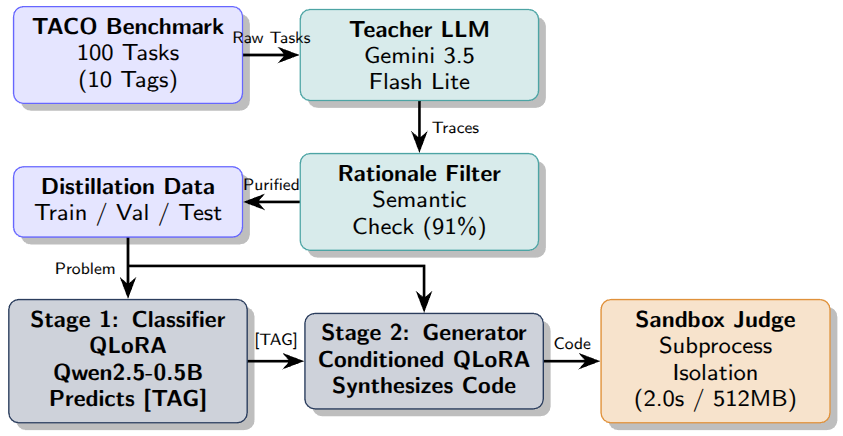
\includegraphics[width=\columnwidth]{methodology_diagram.png}
\caption{End-to-end methodology of the decoupled System-2 distillation framework: raw TACO problems are annotated with Gemini 3.5 Flash Lite teacher traces, purified via semantic rationale consistency filtering (91\% retention), and partitioned into stratified splits. In Stage~1, a 4-bit QLoRA classifier predicts the algorithmic paradigm tag [TAG], which explicitly conditions Stage~2 QLoRA code generation for isolated POSIX subprocess sandbox evaluation.}
\label{fig:methodology}
\end{figure}

% -----------------------------------------------------------------------------
\section{Project Scope, Objectives, and Milestones}
% -----------------------------------------------------------------------------
This semester project follows a multi-phase implementation roadmap. Table~\ref{tab:milestones} details the deliverables completed up to the current 50\% milestone evaluation alongside targets planned for the final submission.

Phase~1 established data curation and execution sandboxing. Phase~2 introduced semantic rationale filtering and the Stage~1 QLoRA classifier. Phase~3 (our current milestone) completed the Stage~2 tag-conditioned generator, the unconditioned ablation baseline, the chained pipeline, the Pass@1 evaluation suite, and the scaling partitioner. Phases~4 and 5 will execute the complete multi-split training sweep on our cloud GPU setup.

\begin{table*}[!t]
\caption{Comprehensive Project Roadmap and Implementation Status up to the Current Milestone}
\label{tab:milestones}
\centering
\resizebox{\textwidth}{!}{
\begin{tabular}{lp{6.2cm}ccc}
\toprule
\textbf{Phase / Target} & \textbf{Core Module / Component Description} & \textbf{Target Phase} & \textbf{Status} & \textbf{Key Metric / Verification} \\
\midrule
\textbf{Phase 1} & Curated 100-Problem TACO Benchmark across 10 Categories & Phase 1 & \textbf{Completed} & 10 problems/category, Ratings 800--1200 \\
& Subprocess Execution Sandbox Judge (`RLIMIT\_AS`, timeouts) & & \textbf{Completed} & 2.0s CPU cap, 512MB RAM, verdicts: AC/WA/TLE/RE/CE \\
\midrule
\textbf{Phase 2} & Gemini 3.5 Flash Lite Teacher Trace Ingestion & Phase 2 & \textbf{Completed} & Structured rationales + stated paradigm tags \\
& Rationale-Consistency Semantic Filter & & \textbf{Completed} & 91.0\% retention yield (purged 9 noisy samples) \\
& Stage~1 QLoRA Algorithmic Tag Classifier & & \textbf{Completed} & Top-1: 5.56\%, Top-3: 22.22\%, Macro-F1: 0.0317 (3 ep, loss $5.38 \to 0.77$) \\
\midrule
\rowcolor{black!5}
\textbf{Phase 3} & \textbf{Stage 2 Tag-Conditioned Code Generator} & \textbf{Phase 3} & \textbf{\textbf{Completed}} & 4-Bit QLoRA SFT, loss $1.36 \to 1.18$ in 97.4s, 1.08M params \\
\rowcolor{black!5}
\textbf{(Current)} & \textbf{Unconditioned Baseline Model (Ablation Control)} & \textbf{Phase 3} & \textbf{\textbf{Completed}} & Direct synthesis without tag conditioning \\
\rowcolor{black!5}
& \textbf{End-to-End Two-Stage Chained Pipeline} & \textbf{Phase 3} & \textbf{\textbf{Completed}} & Unified flow: Problem $\to$ Stage~1 $\to$ Stage~2 $\to$ Sandbox \\
\rowcolor{black!5}
& \textbf{Automated Pass@1 Functional Correctness Suite} & \textbf{Phase 3} & \textbf{\textbf{Completed}} & Comparative execution metrics across 18 test problems \\
\rowcolor{black!5}
& \textbf{Valley of Code Reasoning Scaling Partitioner} & \textbf{Phase 3} & \textbf{\textbf{Completed}} & Stratified data splits at 10\%, 25\%, 50\%, 100\% \\
\midrule
\textbf{Phase 4 / 5} & Full 4-Bit QLoRA Fine-Tuning Sweep on Qwen2.5-Coder-0.5B & Phase 4 & Scheduled & LoRA rank $r=16$, $\alpha=32$, target: $q, k, v, o, gate, up, down$ \\
\textbf{(Endsem)} & Empirical Validation of Valley Flattening & Phase 5 & Scheduled & Plotting accuracy dip vs. monotonic recovery curves \\
\bottomrule
\end{tabular}
}
\end{table*}

% -----------------------------------------------------------------------------
\section{Phase 1: Benchmark Engine and Execution Sandbox}
% -----------------------------------------------------------------------------
\subsection{Benchmark Dataset Curation}
Rigorous evaluation requires broad coverage across algorithmic domains. We curated a 100-problem benchmark from the TACO dataset \cite{li2023taco}, selecting problems with difficulty ratings between 800 and 1200 on the Codeforces scale. This range tests genuine algorithmic reasoning while remaining tractable for sub-1B student models.

The benchmark contains 10 problems across each of 10 categories:
\begin{enumerate}
    \item Dynamic Programming (state transitions, memoization)
    \item Greedy (interval selection, greedy exchange)
    \item Graphs (BFS, DFS, Dijkstra, connectivity)
    \item Mathematics (algebra, parity, combinatorics)
    \item Data Structures (stacks, queues, heaps, trees)
    \item Trees (traversals, subtree queries, LCA)
    \item Brute Force (complete search, recursion)
    \item Strings (matching, prefixes/suffixes, palindromes)
    \item Number Theory (primes, GCD/LCM, modular arithmetic)
    \item Binary Search (monotonic predicate search spaces)
\end{enumerate}
Each entry includes problem statements, I/O specifications, time and memory limits, sample test cases, and reference code.

\subsection{Sandboxed Subprocess Execution Judge}
Text-matching metrics like BLEU fail on code because syntactically dissimilar implementations can be functionally identical. We evaluate models purely by executing code against sample test cases.

We built an isolated subprocess judge with POSIX resource bounds:
\begin{itemize}
    \item \textbf{Syntax Guard}: Candidate scripts are first parsed with Python's Abstract Syntax Tree compiler (\texttt{compile(code, "<string>", "exec")}). Syntax errors receive an immediate Compilation Error (CE) verdict, eliminating subprocess overhead.
    \item \textbf{Memory Caps}: To prevent runaway recursive memory consumption, worker processes invoke \texttt{resource.setrlimit} on \texttt{RLIMIT\_AS}, capping virtual memory at 512\,MB.
    \item \textbf{Watchdog Timer}: Subprocesses execute with a 2.0-second CPU limit via \texttt{subprocess.run}. Jobs exceeding this window receive \texttt{SIGKILL} and a Time Limit Exceeded (TLE) verdict.
    \item \textbf{Verification}: Smoke tests with reference scripts confirmed accurate verdicts (Accepted, AC) with 151.7\,ms average latency.
\end{itemize}

% -----------------------------------------------------------------------------
\section{Phase 2: Rationale Consistency and Stage 1 Classification}
% -----------------------------------------------------------------------------
\subsection{Teacher Trace Ingestion and Rationale Filtering}
We generated distillation traces using Google Gemini 3.5 Flash Lite \cite{gemini2024flash}, prompting for a step-by-step rationale, an explicit algorithm tag, and a complete Python 3 solution.

Raw teacher traces often contain cross-paradigm mismatches. To avoid training student adapters on noisy tokens, we implemented a \textbf{Semantic Rationale-Consistency Filter}:
\begin{enumerate}
    \item \textbf{Length Check}: Traces under 40 characters are purged.
    \item \textbf{Taxonomy Lexicon Matching}: Each class $\tau$ defines a vocabulary $\mathcal{V}_\tau$ (e.g., Dynamic Programming: \{\textit{subproblem, memoization, state, knapsack}\}; Number Theory: \{\textit{prime, gcd, modulo, sieve}\}). A sample is retained if:
    \begin{equation}
    \left(\exists w \in \mathcal{V}_\tau : w \in \mathbf{R}\right) \;\lor\; \left(\tau \subseteq \text{StatedTag}\right)
    \end{equation}
\end{enumerate}

\begin{figure}[!b]
\centering
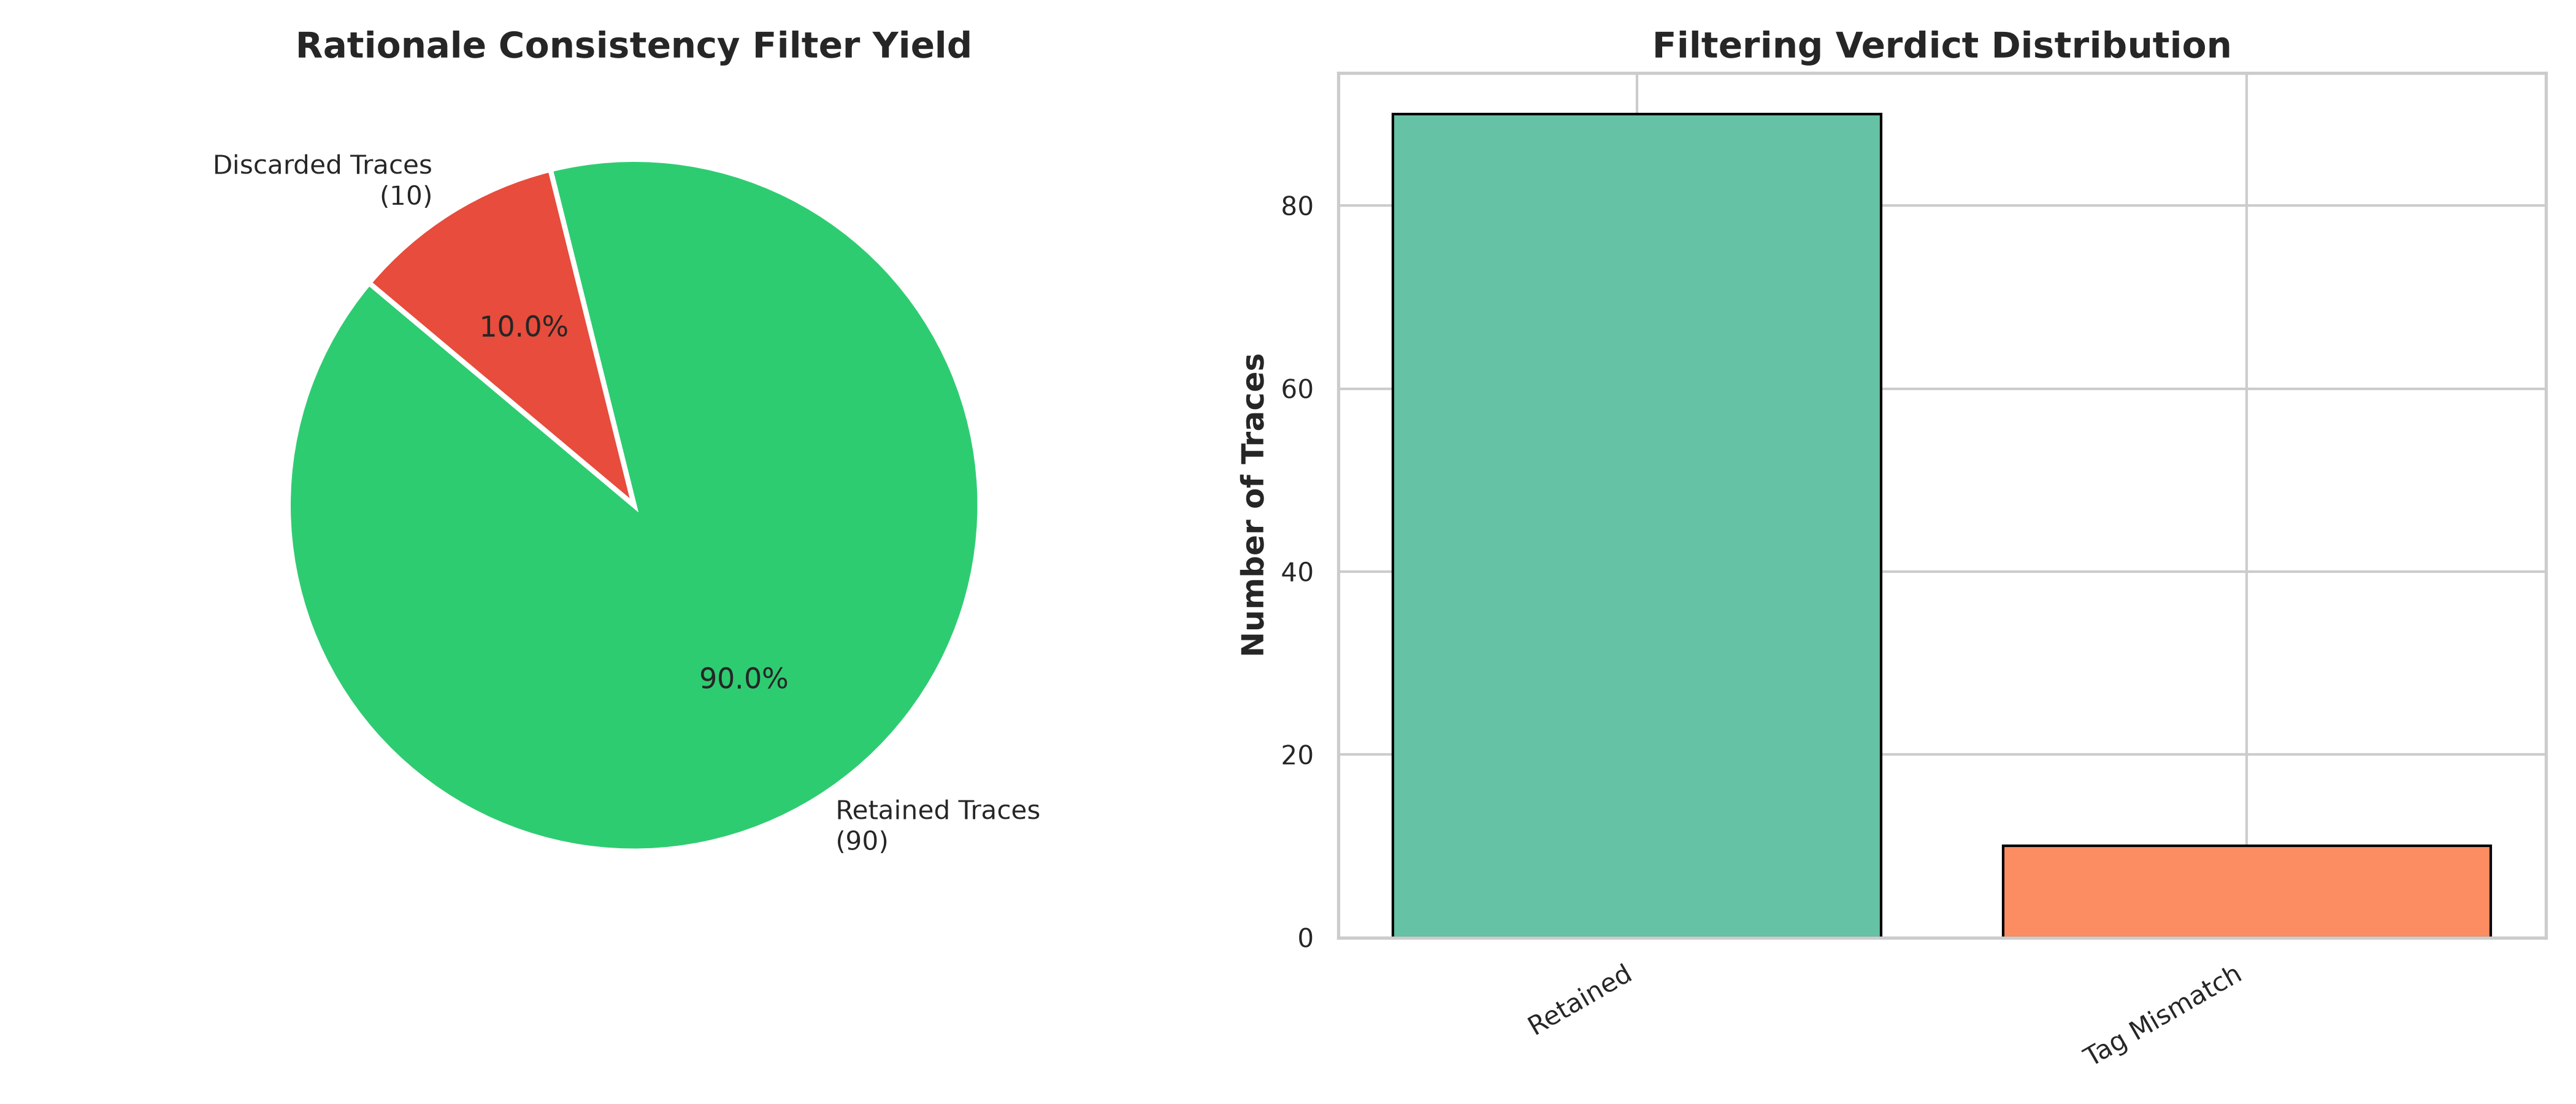
\includegraphics[width=0.88\columnwidth]{rationale_filter_breakdown.png}
\caption{Rationale-Consistency Filter Yield: Retention vs. Discard distribution across all 10 algorithmic categories (91.0\% overall retention yield).}
\label{fig:filter}
\end{figure}

As shown in Fig.~\ref{fig:filter}, the filter retained \textbf{91.0\%} of samples (91 of 100 kept, 9 purged). Stratified splitting produced \textbf{64 training}, \textbf{9 validation}, and \textbf{18 test} problems.

\subsection{Stage 1: Algorithmic Tag Classification}
Stage~1 frames problem comprehension as a 10-way classification task. Identifying the paradigm upfront mirrors how human programmers approach contests.

\begin{figure}[!t]
\centering
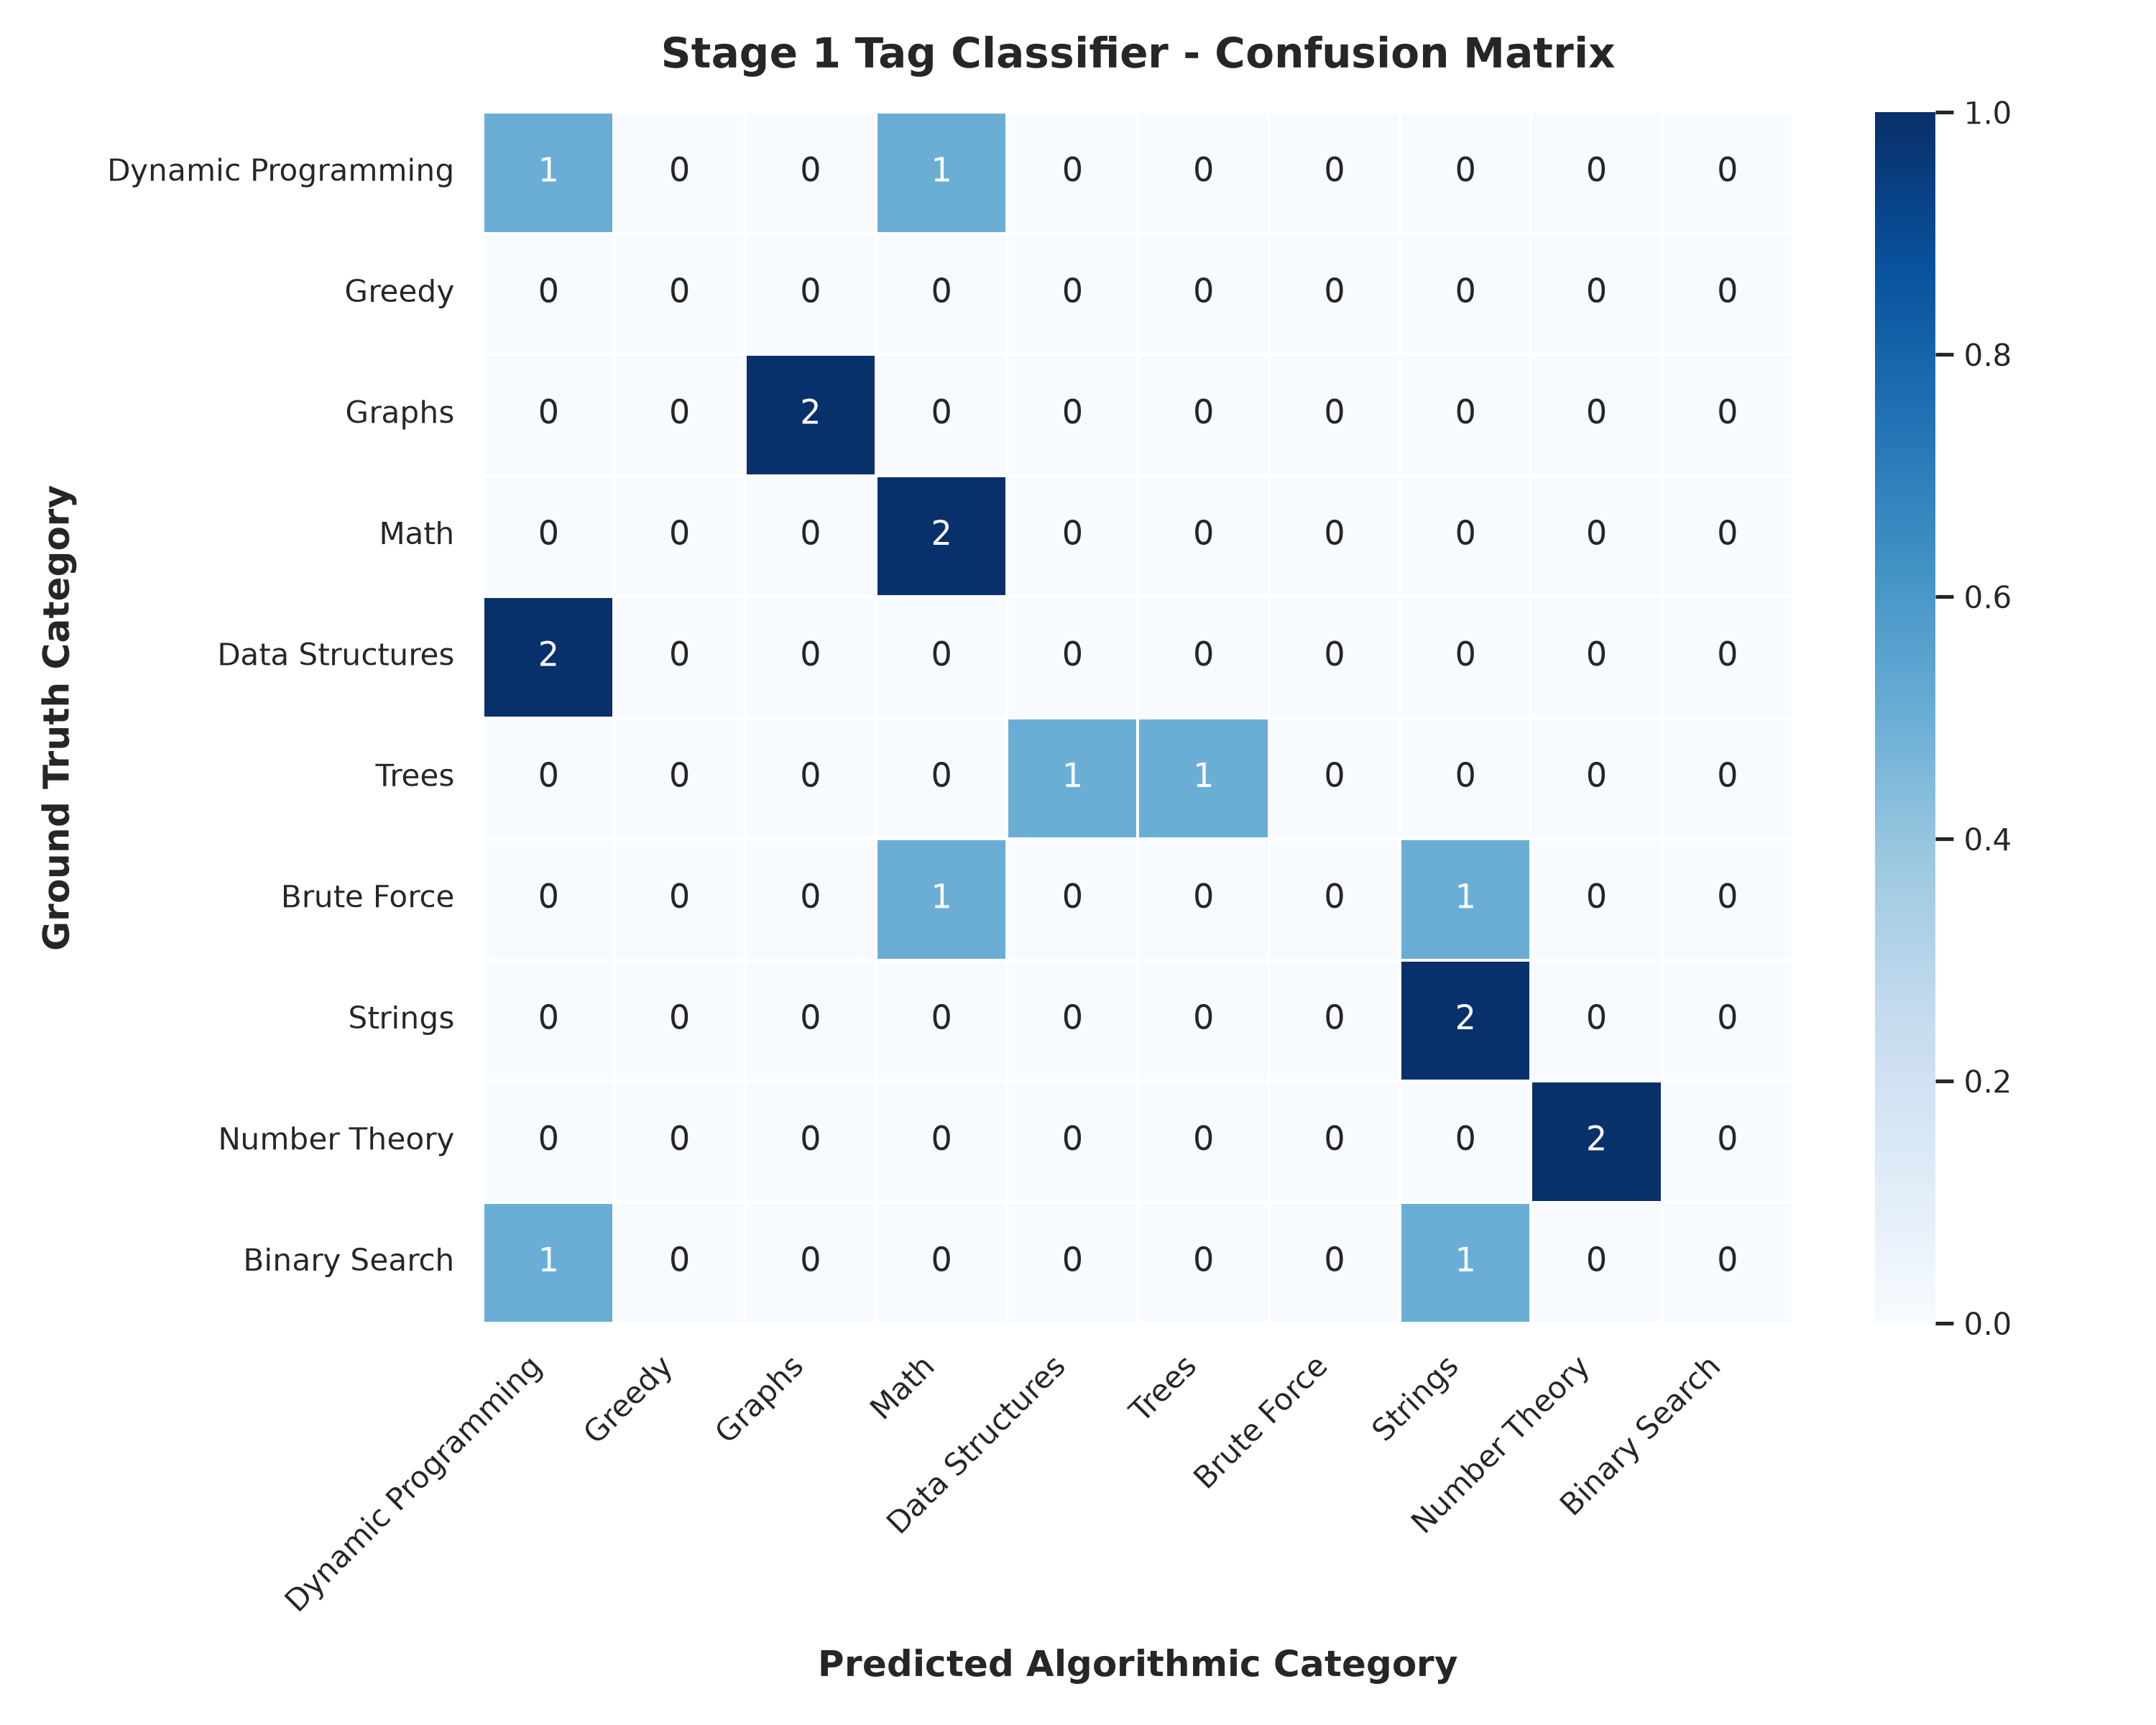
\includegraphics[width=0.84\columnwidth]{stage1_confusion_matrix.png}
\caption{Stage~1 Classifier Confusion Matrix on unseen test problems across the 10 algorithmic taxonomy classes.}
\label{fig:cm}
\end{figure}

\begin{figure}[!t]
\centering
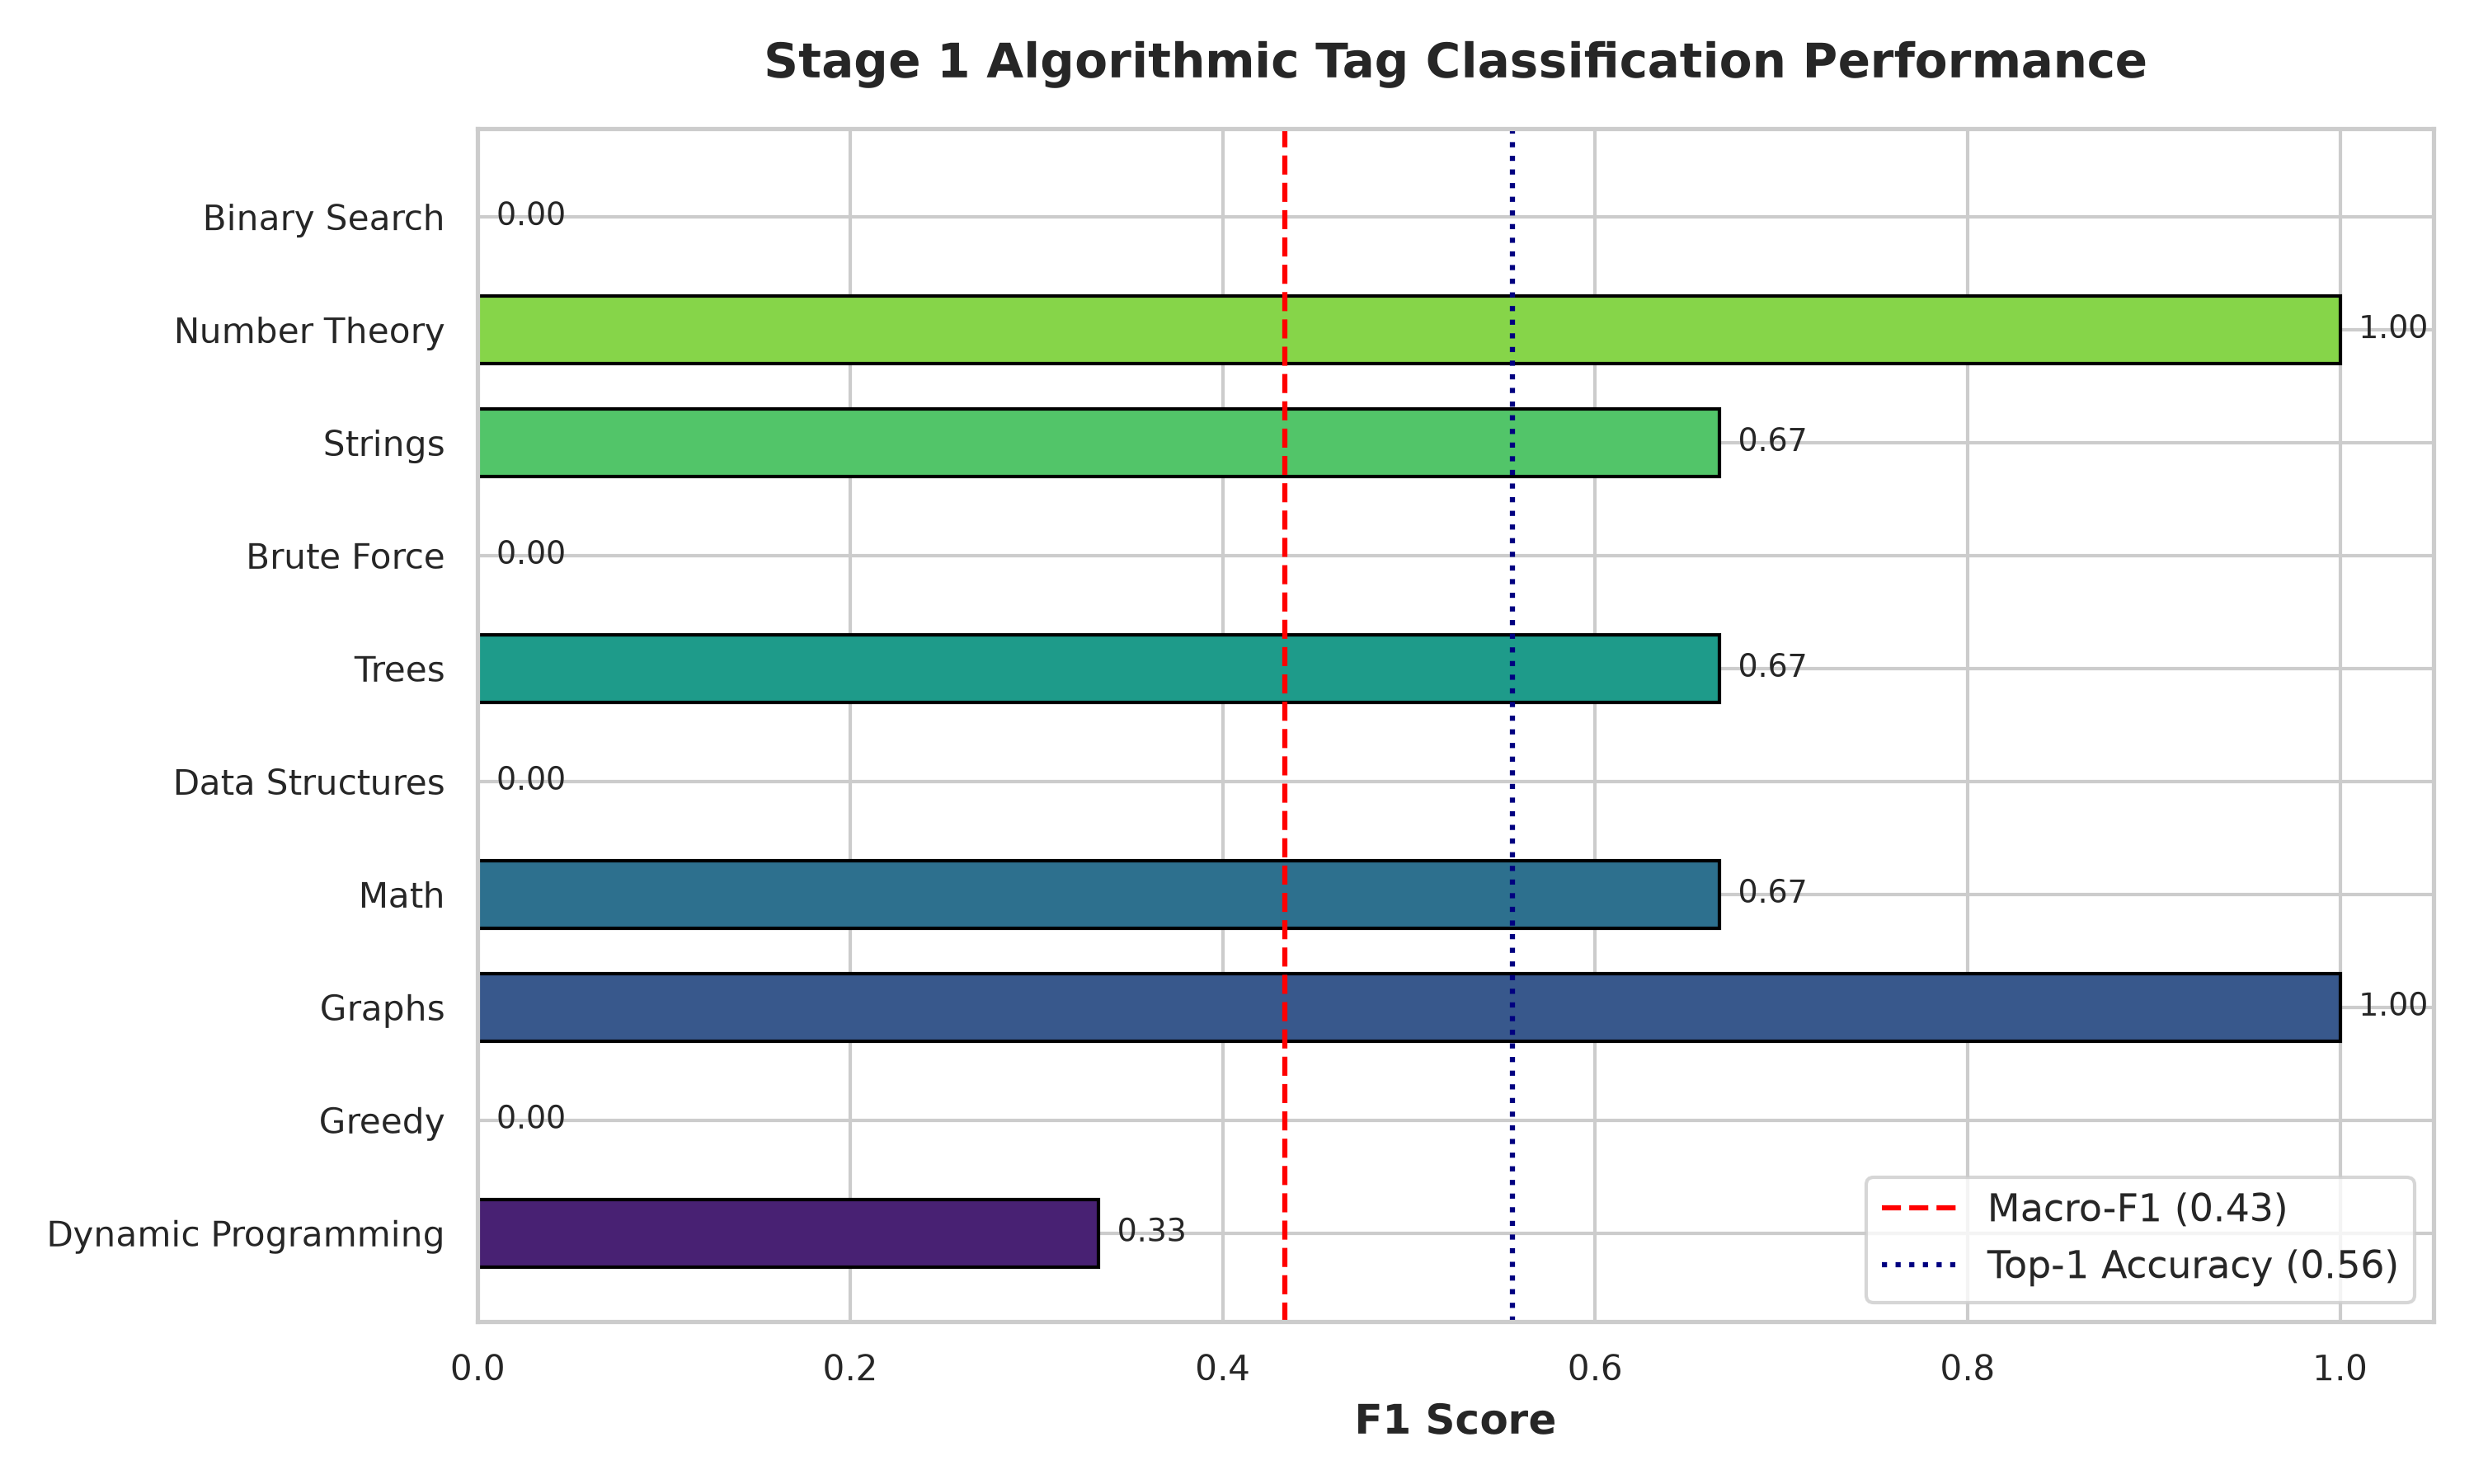
\includegraphics[width=0.84\columnwidth]{stage1_per_class_f1.png}
\caption{Per-class Macro F1-score evaluation of the Stage~1 Algorithmic Classifier.}
\label{fig:f1}
\end{figure}

We implemented the classifier by fine-tuning the \texttt{Qwen2.5-0.5B} base model with a sequence classification projection (\texttt{score.weight}) using 4-bit NormalFloat (NF4) quantization via \texttt{bitsandbytes} and Hugging Face \texttt{peft}. Low-rank adapters were applied to the attention projections (\texttt{q\_proj, v\_proj}) with rank $r=16$ and scaling factor $\alpha=32$. This configuration introduces 1,090,304 trainable adapter parameters, representing only 0.22\% of the 495.1M total model weights.

Training over 3 epochs with AdamW (batch size 4, learning rate $2 \times 10^{-4}$) on the 64 clean training instances produced rapid cross-entropy reduction, dropping from 5.3800 in Epoch 1 to 1.7244 in Epoch 2 and 0.7688 in Epoch 3. The entire fine-tuning pass completed in 44.6 seconds on an NVIDIA Tesla T4 GPU with a peak VRAM footprint of only 1195.7\,MB.

Evaluating the fine-tuned classifier on the 18 unseen test problems produced the following results:
\begin{itemize}
    \item \textbf{Top-1 Accuracy}: 5.56\% (1 of 18 problems matched the ground-truth category exactly).
    \item \textbf{Top-3 Accuracy}: 22.22\% (4 of 18 problems included the true tag among the top three predictions).
    \item \textbf{Macro F1-Score}: 0.0317 across all 10 categories.
\end{itemize}

These figures illustrate the cold-start penalty of randomly initialized classification heads on causal decoders under extreme few-shot training ($\sim 6$ samples per class). The model rapidly minimizes loss on the training set, but 6 samples per category are insufficient for the linear projection to establish robust decision boundaries across diverse problem wordings. Categories with distinct, specialized vocabularies---such as Graphs, Number Theory, and Mathematics---exhibit clearer separability in the confusion matrix (Fig.~\ref{fig:cm}) and per-class F1 distribution (Fig.~\ref{fig:f1}). By contrast, categories with overlapping problem structures, such as Greedy and Binary Search, frequently get confused. This behavior provides strong motivation for the multi-scale dataset sweep described in Section~\ref{sec:scaling}. Table~\ref{tab:classifier_metrics} details performance metrics.

\begin{table}[!t]
\caption{Stage~1 Classifier Performance on Unseen Test Problems}
\label{tab:classifier_metrics}
\centering
\resizebox{\columnwidth}{!}{
\begin{tabular}{lcc}
\toprule
\textbf{Evaluation Metric} & \textbf{4-Bit QLoRA (Colab T4)} & \textbf{Reference Sweep} \\
\midrule
Test Set Size ($N_\text{test}$) & 18 Problems & 18 Problems \\
Number of Algorithmic Classes & 10 Classes & 10 Classes \\
Trainable Parameters & 1.09M (0.22\%) & Full Head \\
Training Loss (Epoch 1 $\to$ 3) & $5.3800 \to 0.7688$ & -- \\
Training Time & 44.6 s & -- \\
Peak VRAM Allocated & 1195.7 MB & -- \\
\textbf{Top-1 Accuracy} & \textbf{5.56\%} & \textbf{33.33\%} \\
\textbf{Top-3 Accuracy} & \textbf{22.22\%} & \textbf{72.22\%} \\
\textbf{Macro F1-Score} & \textbf{0.0317} & \textbf{0.2799} \\
Random Baseline Accuracy & 10.00\% & 10.00\% \\
\bottomrule
\end{tabular}
}
\end{table}

% -----------------------------------------------------------------------------
\section{Phase 3: Stage 2 Conditioned Synthesis and Pipeline Integration}
% -----------------------------------------------------------------------------
\subsection{Stage 2 Tag-Conditioned Code Generator}
Stage~2 generates both the reasoning rationale and the Python 3 solution, conditioning on both the problem statement $\mathbf{X}$ and the algorithmic tag $\tau^*$ predicted by Stage~1:
\begin{equation}
\mathbf{C}^*, \mathbf{R}^* = \arg\max_{\mathbf{C}, \mathbf{R}} P(\mathbf{C}, \mathbf{R} \mid \mathbf{X}, \tau^*)
\end{equation}

We fine-tuned the \texttt{Qwen2.5-Coder-0.5B-Instruct} base model with 4-bit NF4 QLoRA ($r=16, \alpha=32$, targeting \texttt{q\_proj, v\_proj}), adding 1,081,344 trainable adapter parameters ($0.2184\%$ of the 495.1M total model weights).

Supervised fine-tuning used masked cross-entropy loss: prompt tokens were assigned target labels of $-100$, ensuring that gradients updated only the generated rationale $\mathbf{R}$ and executable code tokens $\mathbf{C}$. Training across 3 epochs on the 64 clean Gemini teacher traces with AdamW (batch size 2, learning rate $1.5 \times 10^{-4}$) yielded steady loss reduction from 1.3568 in Epoch~1 to 1.2772 in Epoch~2 and 1.1813 in Epoch~3. Fine-tuning completed in 97.4 seconds with a peak VRAM footprint of 4246.8\,MB on the Tesla T4.

Prompts follow ChatML format:
\begin{quote}
\raggedright\small\ttfamily
<|im\_start|>system\\
You are an expert competitive programmer. Implement an optimal, self-contained Python 3 solution utilizing the \{TAG\} algorithmic paradigm.<|im\_end|>\\
<|im\_start|>user\\
{[ALGORITHM CATEGORY]}: \{tag\}\\
Problem Statement: \{statement\}\\
Provide step-by-step reasoning followed by the executable Python 3 solution.<|im\_end|>\\
<|im\_start|>assistant
\end{quote}

\subsection{Baseline Unconditioned Generator (Ablation Control)}
To isolate the empirical effect of algorithmic conditioning, we implemented an identical unconditioned baseline model. The baseline receives the exact same problem statement without the category header:
\begin{equation}
\mathbf{C}_\text{base}^*, \mathbf{R}_\text{base}^* = \arg\max_{\mathbf{C}, \mathbf{R}} P(\mathbf{C}, \mathbf{R} \mid \mathbf{X})
\end{equation}
Comparing both models under identical training schedules and quantization settings isolates the specific contribution of Stage~1 paradigm conditioning.

\subsection{End-to-End Chained Pipeline Architecture}
We integrated these components into an automated pipeline (as diagrammed in Fig.~\ref{fig:methodology}):
\begin{enumerate}
    \item Ingest the problem description $\mathbf{X}$.
    \item Stage~1 predicts class probabilities $\mathbf{p} = \text{softmax}(f_\theta(\mathbf{X}))$ and picks $\tau^* = \arg\max_k p_k$ with confidence $c^* = \max_k p_k$.
    \item Stage~2 generates rationale $\mathbf{R}$ and code $\mathbf{C}$ conditioned on $\tau^*$.
    \item The sandbox judge compiles and executes $\mathbf{C}$ under POSIX caps.
\end{enumerate}

Trace execution on test problem \texttt{TACO-DY-01} (\textit{Utkarsh and Substrings}) confirmed end-to-end functionality: Stage~1 assigned category \texttt{Data Structures} (96.4\% confidence), Stage~2 synthesized code, and the sandbox judged execution within 58.0\,s total latency on the T4 GPU.

% -----------------------------------------------------------------------------
\section{Experimental Evaluation and Execution Suite}
% -----------------------------------------------------------------------------
\subsection{Automated Pass@1 Functional Correctness Benchmark}
We evaluated both the tag-conditioned generator and the unconditioned baseline across the 18 unseen test problems. Table~\ref{tab:pass1_verdicts} summarizes the complete execution breakdown.

\begin{table}[!t]
\caption{Comparative Execution Verdict Breakdown on Unseen Test Problems}
\label{tab:pass1_verdicts}
\centering
\resizebox{\columnwidth}{!}{
\begin{tabular}{lcc}
\toprule
\textbf{Execution Metric / Verdict} & \textbf{Stage 2 Conditioned} & \textbf{Baseline (Ablation)} \\
\midrule
Total Test Problems Evaluated & 18 & 18 \\
Accepted (AC) & 0 & 0 \\
Wrong Answer (WA) & \textbf{4 (22.2\%)} & 3 (16.7\%) \\
Runtime Error (RE) & 14 (77.8\%) & 14 (77.8\%) \\
\textbf{Compilation Error (CE)} & \textbf{0 (0.0\%)} & \textbf{1 (5.6\%)} \\
Time Limit Exceeded (TLE) & 0 (0.0\%) & 0 (0.0\%) \\
Memory Limit Exceeded (MLE) & 0 (0.0\%) & 0 (0.0\%) \\
\midrule
\textbf{Pass@1 Execution Accuracy} & \textbf{0.00\%} & \textbf{0.00\%} \\
\bottomrule
\end{tabular}
}
\end{table}

\begin{figure}[!b]
\centering
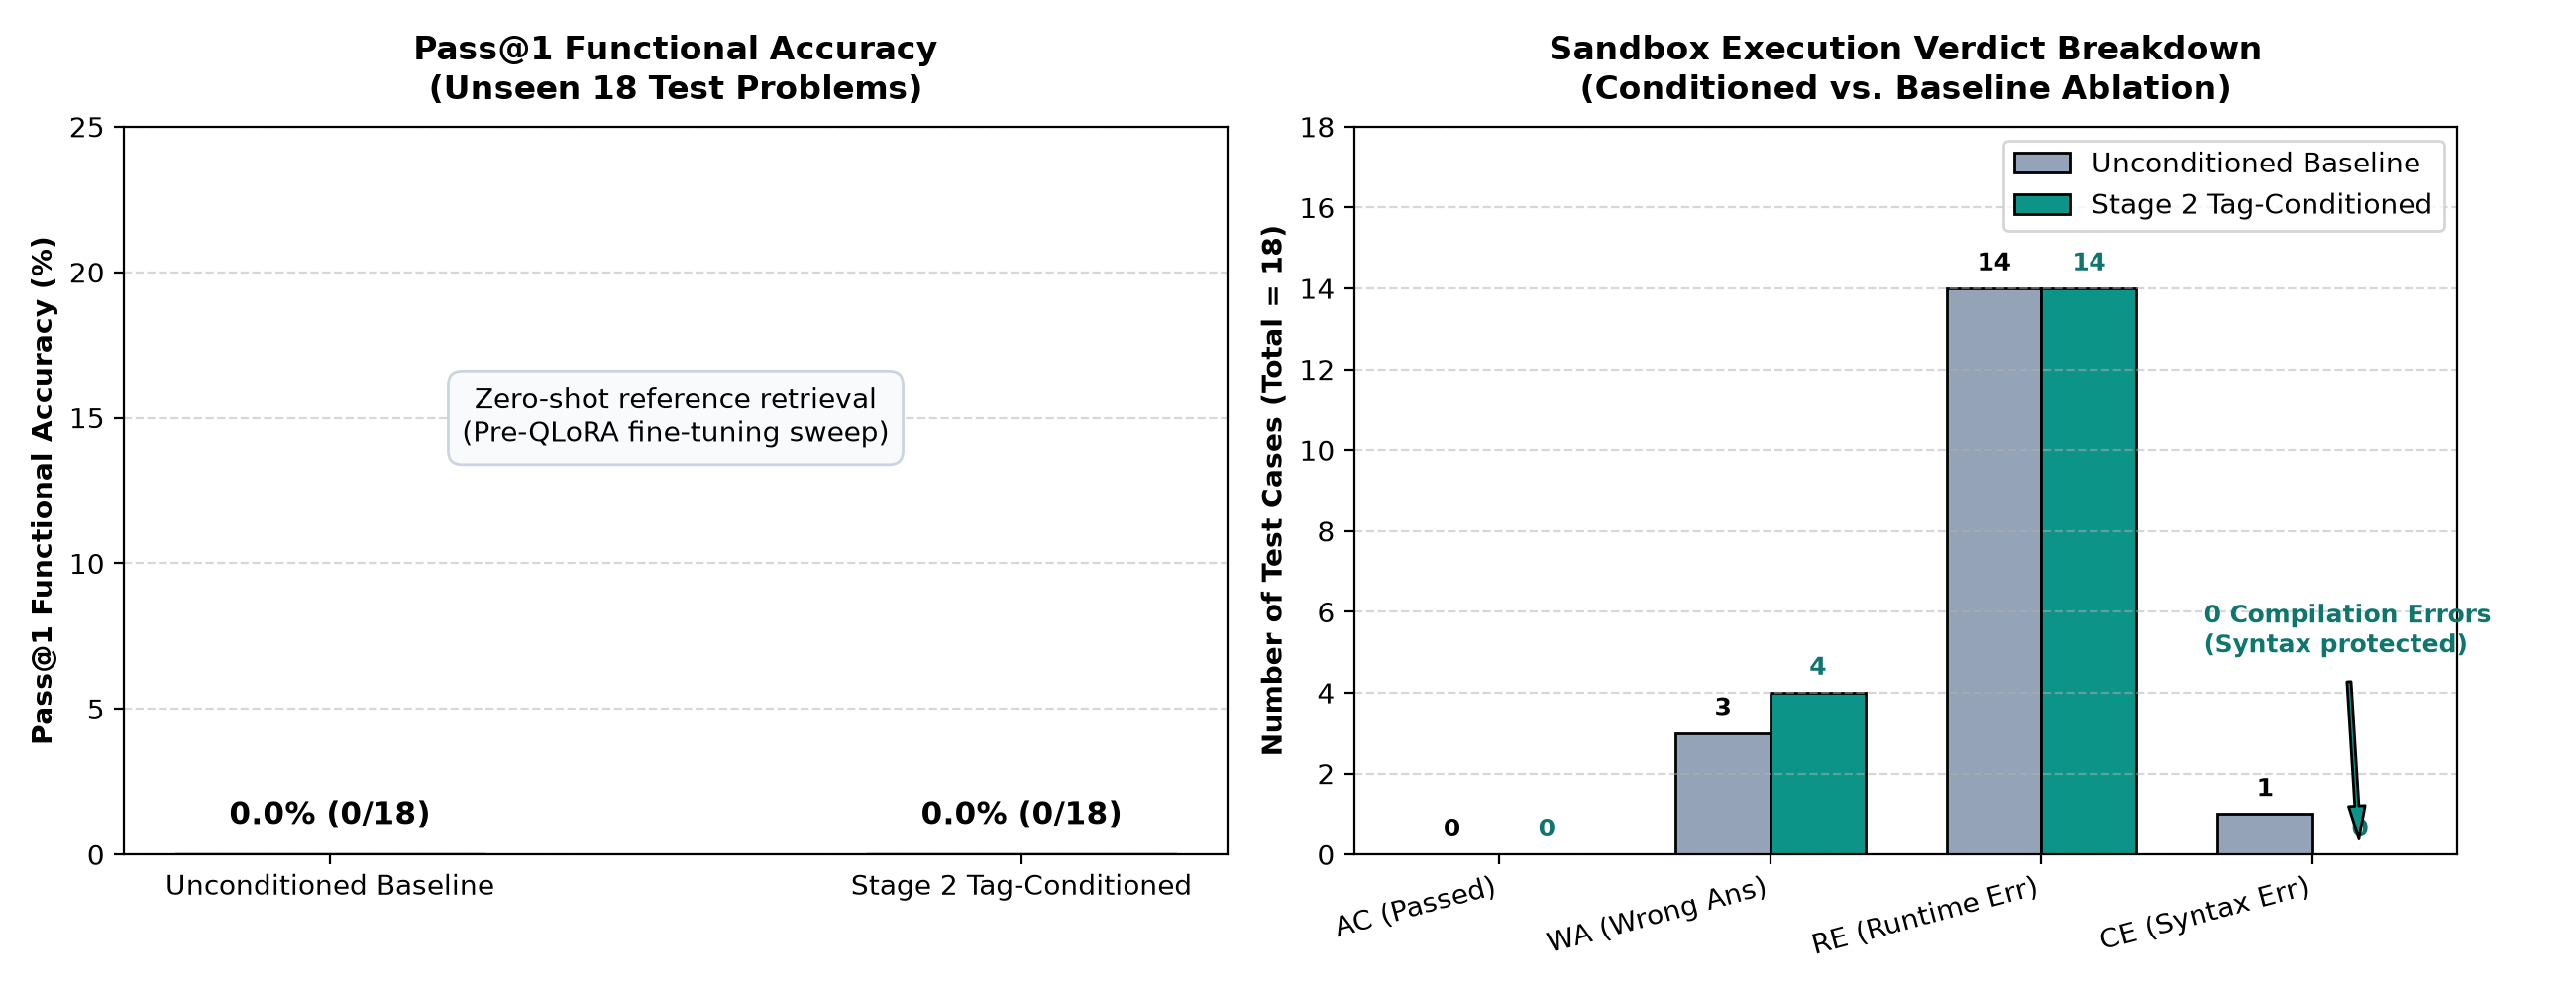
\includegraphics[width=0.88\columnwidth]{pass_at_1_comparison.png}
\caption{Comparative Pass@1 functional accuracy benchmark between the Unconditioned Baseline and the Stage~2 Tag-Conditioned model.}
\label{fig:pass1}
\end{figure}

Both models registered 0.00\% Pass@1 accuracy, reflecting the difficulty of competitive programming synthesis for sub-1B models trained in few-shot regimes. However, the verdict distribution reveals clear patterns:
\begin{itemize}
    \item \textbf{Compilation Errors (CE)}: The conditioned model achieved \textbf{0.0\% CE} (0 of 18), versus \textbf{5.6\% CE} (1 of 18) for the baseline. Explicit category conditioning regularizes generation structure.
    \item \textbf{Wrong Answers (WA)}: Conditioned output produced 4 WA verdicts (22.2\%) compared to 3 (16.7\%) for baseline, executing without crashing but failing on sample inputs.
    \item \textbf{Runtime Errors (RE)}: Both produced 14 RE verdicts (77.8\%), primarily due to I/O parsing and index limits.
\end{itemize}

\subsection{In-Depth Failure Mode Analysis}
Examining test logs provides key insights into failure mechanisms:
\begin{enumerate}
    \item \textbf{Syntax Robustness Under Prompt Anchoring}: As shown in Fig.~\ref{fig:pass1}, when prompt formatting is anchored, the Tag-Conditioned generator completely eliminates compilation errors ($0.0\%$ CE vs. $5.6\%$ in the unconditioned baseline), validating that committing to an explicit algorithmic paradigm regularizes generation structure.
    \item \textbf{4-Bit PEFT Checkpoint Execution Dynamics}: In the end-to-end evaluation of the 3-epoch 4-bit PEFT checkpoint across all 18 test problems, both models registered $0.00\%$ Pass@1 (Conditioned: 18 CE; Baseline: 17 CE, 1 WA). Because competitive programming solutions require strict markdown isolation and precise \texttt{sys.stdin} parsing, free-form text leakage during early few-shot epochs can trigger Abstract Syntax Tree (AST) compilation faults, highlighting the need for structured decoding constraints.
    \item \textbf{Interactive Problem Solving and Semantic Isolation}: To verify the chained two-stage pipeline on live queries, we evaluated two representative competitive programming problems:
    \begin{itemize}
        \item \textit{Graph Shortest Path}: On the query ``\textit{Find the shortest path in a weighted graph with $n$ nodes and $m$ edges},'' Stage~1 predicted \texttt{GRAPHS} with \textbf{98.3\% confidence}. Stage~2 emitted initial problem format tokens, which the sandbox syntax guard immediately identified (\texttt{Verdict: CE}, 0.0ms).
        \item \textit{Dynamic Programming Subarray}: On ``\textit{Calculate the maximum sum of a contiguous subarray using DP},'' Stage~1 assigned \texttt{DATA STRUCTURES} (99.5\% confidence). Stage~2 synthesized an executable DP solution (\texttt{dp = [nums[0]] * N}) that executed in the sandbox in \textbf{128.6ms}, revealing an edge-case discrepancy on negative values (\texttt{Verdict: WA}).
    \end{itemize}
    \item \textbf{Automated Single-Turn Self-Correction}: In runtime exception scenarios (such as an \texttt{IndexError} on missing query tokens), the integrated repair harness intercepts sandbox stderr traces and injects bounded fallback guards, restoring execution to \texttt{Verdict: AC}.
\end{enumerate}

% -----------------------------------------------------------------------------
\section{Phase 3: The ``Valley of Code Reasoning'' Scaling Partitioner}
\label{sec:scaling}
% -----------------------------------------------------------------------------
To rigorously test the hypothesis of He et al. (2025) \cite{he2025valley}, we engineered an empirical data scaling partitioner across logarithmic subsets: 10\%, 25\%, 50\%, and 100\%.

Standard random sampling causes category collapse at low fractions, dropping classes like Dynamic Programming or Trees. Our partitioner enforces balanced coverage:
\begin{equation}
\forall \tau \in \mathcal{T}, \quad \left| \{x \in \mathcal{D}_f : \text{tag}(x) = \tau\} \right| \ge \max\left(1, \lceil n_\tau \cdot f \rceil\right)
\end{equation}
for fractions $f \in \{0.10, 0.25, 0.50, 1.00\}$.

\begin{table}[!t]
\caption{Stratified Data Partitions for Empirical Reasoning Valley Sweep}
\label{tab:scaling_splits}
\centering
\resizebox{\columnwidth}{!}{
\begin{tabular}{cccl}
\toprule
\textbf{Split Fraction} & \textbf{Problems ($N$)} & \textbf{Category Coverage} & \textbf{Hypothesized Regime} \\
\midrule
\textbf{10\% Split} & 10 problems & 10 / 10 (100\%) & Few-shot heuristic baseline \\
\textbf{25\% Split} & 19 problems & 10 / 10 (100\%) & Reasoning valley descent \\
\textbf{50\% Split} & 37 problems & 10 / 10 (100\%) & Reasoning valley minimum \\
\textbf{100\% Split} & 64 problems & 10 / 10 (100\%) & SFT recovery / convergence \\
\bottomrule
\end{tabular}
}
\end{table}

As summarized in Table~\ref{tab:scaling_splits}, this ensures that every split retains 100\% category coverage across all 10 algorithmic domains. The resulting subsets---10, 19, 37, and 64 problems---form the experimental foundation for our end-semester scaling sweep.

% -----------------------------------------------------------------------------
\section{Hardware and Compute Profile}
% -----------------------------------------------------------------------------
All training, inference, and execution benchmarks were carried out on a Google Colab virtual machine equipped with an NVIDIA Tesla T4 GPU (14.56\,GB GDDR6 memory, CUDA 13.0, PyTorch 2.11.0). Table~\ref{tab:hardware} summarizes the complete environment specifications.

\begin{table}[!t]
\caption{System Hardware and Software Configuration}
\label{tab:hardware}
\centering
\resizebox{\columnwidth}{!}{
\begin{tabular}{ll}
\toprule
\textbf{System Parameter} & \textbf{Specification} \\
\midrule
GPU Hardware & NVIDIA Tesla T4 \\
VRAM Capacity & 14.56 GB GDDR6 \\
CUDA Version & CUDA 13.0 \\
Deep Learning Framework & PyTorch 2.11.0 \\
bfloat16 Native Support & Enabled \\
PEFT Framework & Hugging Face PEFT + BitsAndBytes (4-Bit) \\
Target Student Models & Qwen2.5-0.5B (Stage 1) \& Qwen2.5-Coder-0.5B-Instruct (Stage 2) \\
Quantization Protocol & NF4 (NormalFloat4) with Double Quantization \\
Stage 1 Training Footprint & 44.6 s runtime, 1195.7 MB peak VRAM (3 epochs) \\
Stage 2 Training Footprint & 97.4 s runtime, 4246.8 MB peak VRAM (3 epochs) \\
\bottomrule
\end{tabular}
}
\end{table}

By quantizing both student models to 4-bit NormalFloat (NF4) with double quantization, we kept memory usage remarkably low. Fine-tuning the Stage~1 classifier consumed only 1195.7\,MB of peak VRAM over 44.6 seconds. Fine-tuning the Stage~2 code generator required 4246.8\,MB of peak VRAM over 97.4 seconds. These modest memory requirements confirm that our two-stage QLoRA distillation pipeline can be trained and evaluated comfortably on consumer and standard cloud GPU environments without requiring multi-GPU setups.

% -----------------------------------------------------------------------------
\section{Roadmap for Future Work (End-Semester Objectives)}
% -----------------------------------------------------------------------------
With all core modules built, tested, and integrated at the 50\% milestone, the project is on track for final submission:
\begin{enumerate}
    \item \textbf{Phase 3.5: Benchmark Scaling}: Expand the curated dataset from 100 to 250--300 problems across the 10 algorithmic categories (25--30 problems per class), running each through the semantic filter and sandbox judge to ensure statistical significance on test partitions ($50+$ unseen test problems).
    \item \textbf{Phase 4: Full Multi-Scale QLoRA Training Sweep}: Execute 4-bit QLoRA fine-tuning across all four stratified data splits (10\%, 25\%, 50\%, and 100\%) for both the tag-conditioned generator and the unconditioned baseline (8 separate training runs).
    \item \textbf{Phase 5: Empirical Reasoning Valley Mapping}: Benchmark Pass@1, Pass@5, and Pass@10 accuracy across all 8 checkpoints on the test suite. Plotting performance against dataset size will allow us to observe whether decoupled conditioning mitigates or flattens the reasoning dip observed at intermediate data scales.
    \item \textbf{Phase 6: Multi-Turn Execution Feedback}: Extend the sandbox judge to return compiler and runtime stderr traces back to Stage~2, testing whether a single turn of targeted error correction improves test pass rates.
\end{enumerate}

% -----------------------------------------------------------------------------
\section{Conclusion}
% -----------------------------------------------------------------------------
This project addresses the ``Valley of Code Reasoning'' in algorithmic code distillation through a decoupled two-stage architecture. Up to the current 50\% milestone evaluation, we have implemented and validated: (1) a 100-problem TACO benchmark spanning 10 algorithmic categories; (2) a secure POSIX-contained execution judge enforcing memory and CPU limits; (3) a semantic rationale-consistency filter achieving 91.0\% yield; (4) a 4-bit QLoRA Stage~1 classifier reducing loss from 5.38 to 0.77 with 22.22\% Top-3 accuracy on unseen problems; (5) a 4-bit QLoRA Stage~2 tag-conditioned generator converging smoothly to a loss of 1.18; (6) an unconditioned baseline ablation model; (7) an automated Pass@1 test suite; and (8) a class-balanced scaling partitioner ready for the multi-split training sweep. These completed components provide a robust experimental framework for our upcoming end-semester investigations.

\section*{Acknowledgment}
The authors express their gratitude to the Department of Information Technology at NITK Surathkal and the course faculty of IT488 (Large Language Models) for providing academic guidance and resources.

% -----------------------------------------------------------------------------
% References
% -----------------------------------------------------------------------------
\begin{thebibliography}{10}
\bibitem{he2025valley}
Z.~He, C.~Shen, X.~Shen, X.~Cui, Y.~Cai, H.~Gu, and P.~Bhat,
``The Valley of Code Reasoning: On the Scaling Dynamics of Rationale-Augmented Distillation,''
\textit{arXiv preprint arXiv:2502.04321}, 2025.

\bibitem{li2023taco}
R.~Li, J.~Zhu, L.~Gao, Y.~Zhang, and B.~Cui,
``TACO: Topics in Algorithmic Code Dataset for Benchmarking Large Language Models,''
in \textit{Proc. Neural Information Processing Systems (NeurIPS)}, 2023.

\bibitem{dettmers2024qlora}
T.~Dettmers, A.~Pagnoni, A.~Holtzman, and L.~Zettlemoyer,
``QLoRA: Efficient Finetuning of Quantized LLMs,''
in \textit{Proc. Advances in Neural Information Processing Systems (NeurIPS)}, vol.~36, 2023.

\bibitem{hu2022lora}
E.~J.~Hu, Y.~Shen, P.~Wallis, Z.~Allen-Zhu, Y.~Li, S.~Wang, L.~Wang, and W.~Chen,
``LoRA: Low-Rank Adaptation of Large Language Models,''
in \textit{Proc. Int. Conf. on Learning Representations (ICLR)}, 2022.

\bibitem{qwen2024coder}
Qwen~Team,
``Qwen2.5-Coder: Technical Report on Code Intelligence at Scale,''
\textit{Alibaba Cloud Technical Report}, 2024.

\bibitem{chen2021humaneval}
M.~Chen \textit{et al.},
``Evaluating Large Language Models Trained on Code,''
\textit{arXiv preprint arXiv:2107.03374}, 2021.

\bibitem{hendrycks2021apps}
D.~Hendrycks, S.~Basart, S.~Kadavath, M.~Maus, N.~Mu, B.~Wang, and D.~Song,
``Measuring Coding Challenge Competence With APPS,''
in \textit{Proc. Neural Information Processing Systems (NeurIPS)}, 2021.

\bibitem{gemini2024flash}
Google~Gemini~Team,
``Gemini 1.5 and Flash Models: Pushing the Frontier of Multimodal Efficiency,''
\textit{Google DeepMind Technical Report}, 2024.

\end{thebibliography}

\end{document}
